\chapter{Java内存模型与分配机制}
\label{chp:Java-memory-allocation}

\section*{基本信息}
\sline
\begin{description}
\item[课程名称:] Java应用与开发
\item[授课教师:] 王晓东
\item[授课时间:] 第二周(根据校历,本周有两次课)
\item[参考教材:] 本课程参考教材及资料如下:
  \begin{itemize}
  \item 陈国君主编,Java程序设计基础(第5版),清华大学出版社,2015.5
  \item Bruce Eckel, Thinking in Java (3rd)
  \end{itemize}
\end{description}

\section*{教学目标}

\sline

\begin{enumerate}
\item 理解JVM内存模型,掌握JVM内存构成
\item 理解Java程序的运行过程,学会通过调试模式观察内存的变化
\item 了解Java内存管理,认识垃圾回收
\item 建立编程时高效利用内存、避免内存溢出的理念
\end{enumerate}  

\section*{授课方式}

\sline
\begin{description}
\item[理论课:] 多媒体教学、程序演示
\item[实验课:] 上机编程
\end{description}

\newpage
\section*{教学内容}
\sline

%%%%%%%%%%%%%%%%%%%%%%%%%%%%%%%%%%%%%%%%%%%%%%%%%%%%%%%%%%%%%%
\section{Java内存模型}

\subsection{Java虚拟机(Java Virtual Machine, JVM)}

Java虚拟机的架构如图\ref{fig:jvm-arch}所示。

\begin{figure}[htb]
  \centering
  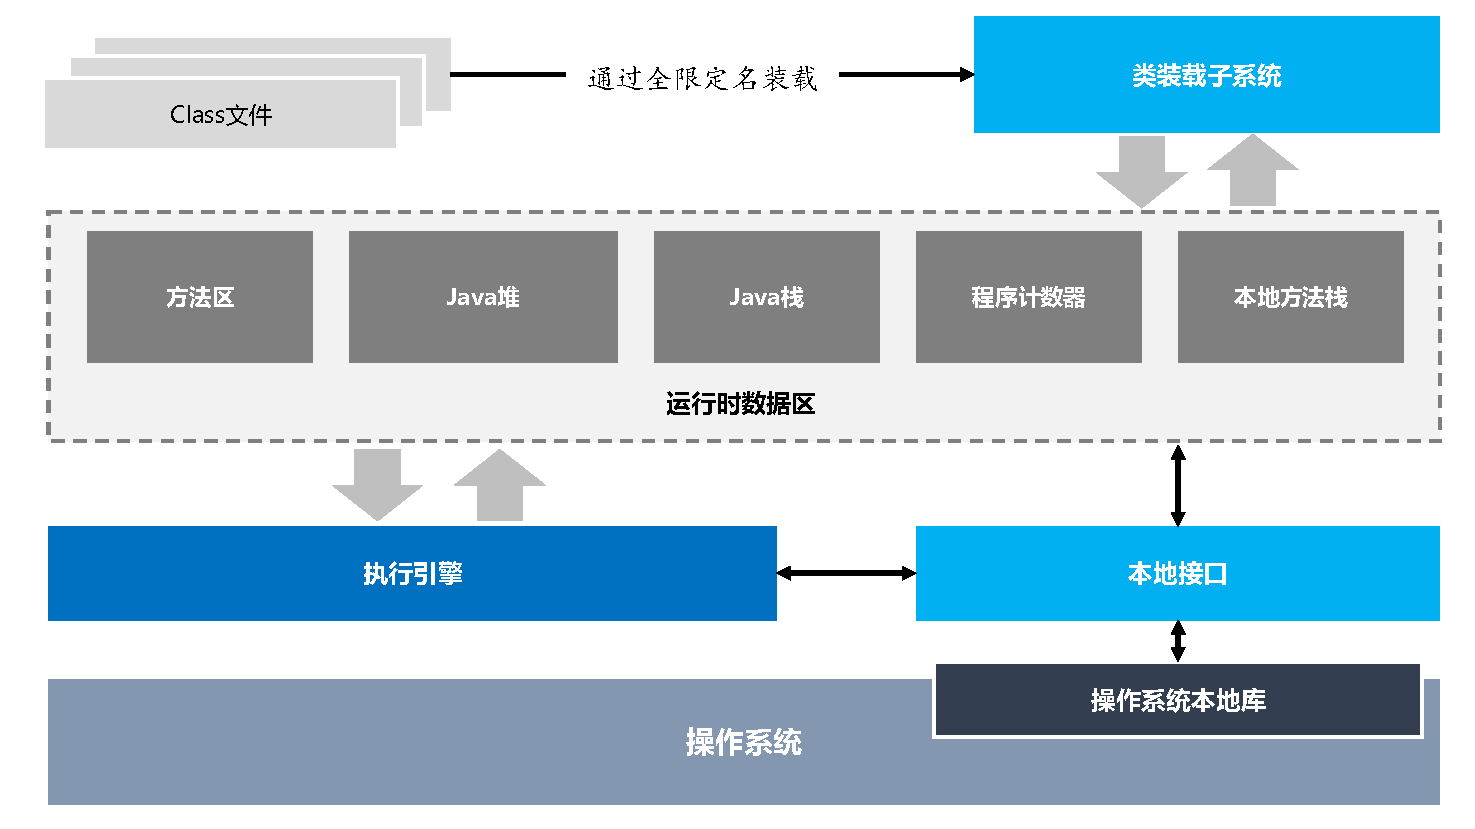
\includegraphics[width=\textwidth]{images/Java-memory-allocation/fig-jvm-arch.pdf}
  \caption{Java虚拟机架构}
  \label{fig:jvm-arch}
\end{figure}

\begin{itemize}
\item Java程序运行在JVM上,JVM是程序与操作系统之间的桥梁。
\item JVM实现了Java的平台无关性。
\item JVM是内存分配的前提。
\end{itemize}

\subsection{JVM内存模型}

\begin{figure}[htb]
  \centering
  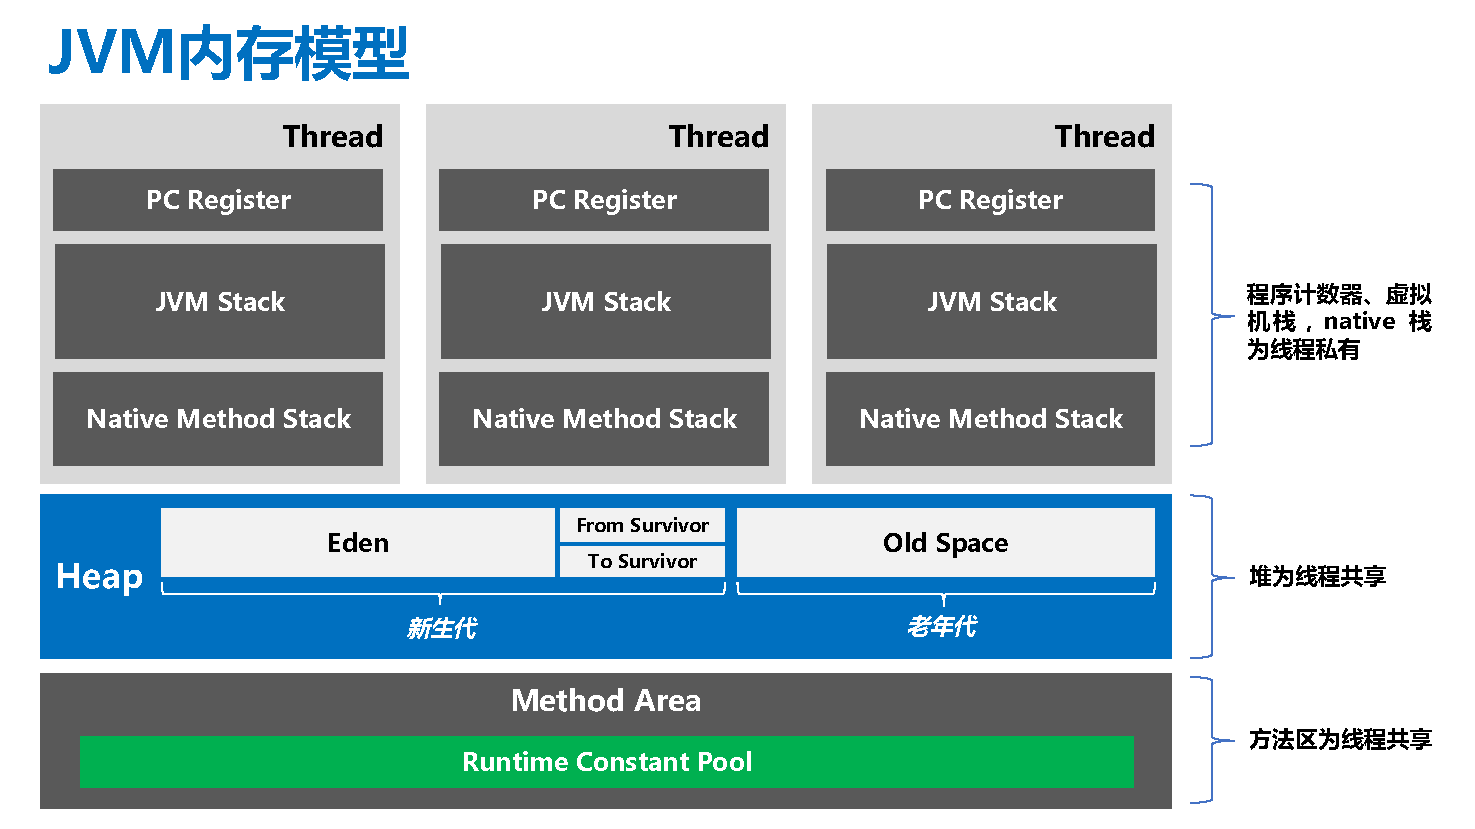
\includegraphics[width=\textwidth]{images/Java-memory-allocation/fig-java-memory-arch.pdf}
  \caption{JVM内存模型}
  \label{fig:java-memory-arch}
\end{figure}

Java程序运行过程会涉及的内存区域包括:

\begin{description}
\item[程序计数器] 当前线程执行的字节码的行号指示器。
\item[栈] 保存局部变量的值,包括:用来保存基本数据类型的值;保存类的实
  例,即堆区对象的引用(指针),也可以用来保存加载方法时的帧。(Stack)
\item[堆] 用来存放动态产生的数据,如new出来的对象和数组\footnote{注意创
    建出来的对象只包含属于各自的成员变量,并不包括成员方法。因为同一个
    类的对象拥有各自的成员变量,存储在各自的堆内存中,但是他们共享该类
    的方法,并不是每创建一个对象就把成员方法复制一次。}。(Heap)
\item[常量池] JVM为每个已加载的类型维护一个常量池,常量池就是这个类型用
  到的常量的一个有序集合。包括直接常量(基本类型、String)和对其他类型、
  方法、字段的符号引用。池中的数据和数组一样通过索引访问,常量池
  在Java程序的动态链接中起了核心作用。(Perm)
\item[代码段] 存放从硬盘上读取的源程序代码。(Perm)
\item[数据段] 存放static定义的静态成员。{\Red (Perm)} 
\end{description}

\section{Java程序内存运行分析}

\subsection{预备知识和所用讲解程序}

\begin{enumerate}
\item 一个Java文件,只要有main入口方法,即可认为这是一个Java程序,可以
  单独编译运行。
\item 无论是普通类型的变量还是引用类型的变量(俗称实例),都可以作为局
  部变量,他们都可以出现在栈中。
\item 普通类型的变量在栈中直接保存它所对应的值,而引用类型的变量保存的
  是一个指向堆区的指针。通过这个指针,就可以找到这个实例在堆区对应的对
  象。因此,{\hei\Red 普通类型变量只在栈区占用一块内存,而引用类型变量
    要在栈区和堆区各占一块内存}。
\end{enumerate}

\samp{Test.java}

\begin{javaCode}
  public class Test {
    public static void main(String[] args) {
      Test test = new Test(); //1
      int data = 9; //2
      BirthDate d1 = new BirthDate(22, 12, 1982); //3
      BirthDate d2 = new BirthDate(10, 10, 1958); //4
      test.m1(data); //5
      test.m2(d1); //7
      test.m3(d2);
    }

    public void m1(int i) {
      i = 1234; //6
    }
    public void m2(BirthDate b) {
      b = new BirthDate(15, 6, 2010); //8
    }
    public void m3(BirthDate b) {
      b.setDay(18);
    }
  }
\end{javaCode}

\subsection{程序调用过程}

\subsubsection{程序调用过程(一)}

\begin{itemize}
\item JVM自动寻找main方法,执行第一句代码,创建一个Test类的实例,在栈中分配一块内存,存放
  一个指向堆区对象的指针110925。
\item 创建一个int型的变量data,由于是基本类型,直接在栈中存放data对应的值9。
\item 创建两个BirthDate类的实例d1、d2,在栈中分别存放了对应的指针指向各自的对象。它们在实
  例化时调用了有参数的构造方法,因此对象中有自定义初始值。
\end{itemize}

\subsubsection{程序调用过程(二)}

\begin{itemize}
\item 调用test对象的m1方法,以data为参数。JVM读取这段代码时,检测到i是局部变量,则会把i放
  在栈中,并且把data的值赋给i。
\end{itemize}

\subsubsection{程序调用过程(三)}

\begin{itemize}
\item 把1234赋值给i。
\end{itemize}

\subsubsection{程序调用过程(四)}

\begin{itemize}
\item m1方法执行完毕,立即释放局部变量i所占用的栈空间。
\end{itemize}

\subsubsection{程序调用过程(五)}

\begin{itemize}
\item 调用test对象的m2方法,以实例d1为参数。JVM检测到m2方法中的b参数为
  局部变量,立即加入到栈中,由于是引用类型的变量,所以b中保存的是d1中的
  指针,此时b和d1指向同一个堆中的对象。在b和d1之间传递是指针。
\end{itemize}

\subsubsection{程序调用过程(六)}

\begin{itemize}
\item m2方法中又实例化了一个BirthDate对象,并且赋给b。在内部执行过程是:
  在堆区new了一个对象,并且把该对象的指针保存在栈中b对应空间,此时实
  例b不再指向实例d1所指向的对象,但是实例d1所指向的对象并无变化,未
  对d1造成任何影响。
\end{itemize}

\subsubsection{程序调用过程(七)}

\begin{itemize}
\item m2方法执行完毕,立即释放局部引用变量b所占的栈空间,注意只是释放了
  栈空间,堆空间要等待自动回收。
\end{itemize}

\subsubsection{程序调用过程(八)}

\begin{itemize}
\item 调用test实例的m3方法,以实例d2为参数。JVM会在栈中为局部引用变
  量b分配空间,并且把d2中的指针存放在b中,此时d2和b指向同一个对象。再调
  用实例b的setDay方法,其实就是调用d2指向的对象的setDay方法。
\item 调用实例b的setDay方法会影响d2,因为二者指向的是同一个对象。
\item m3方法执行完毕,立即释放局部引用变量b。
\end{itemize}

\begin{figure}[htb]
  \begin{minipage}[t]{0.5\linewidth}
    \centering
    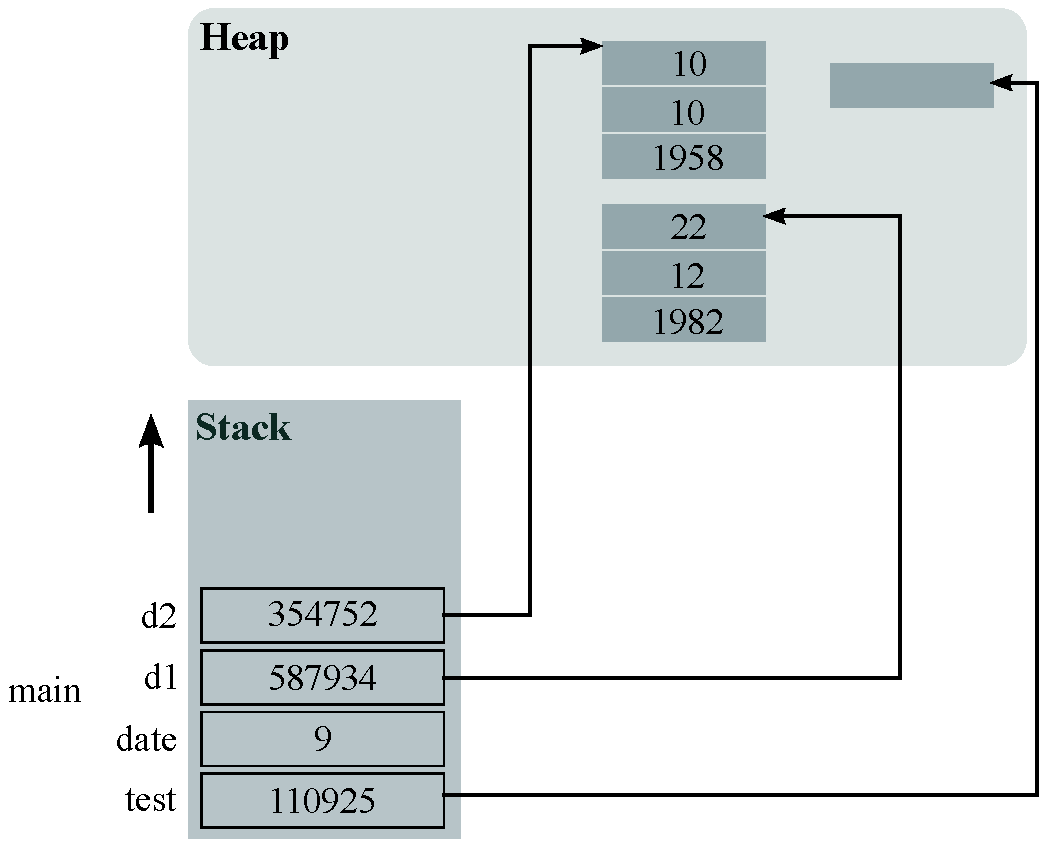
\includegraphics[width=\textwidth]{images/Java-memory-allocation/fig01.pdf}
  \end{minipage}%
  \begin{minipage}[t]{0.5\linewidth}
    \centering
    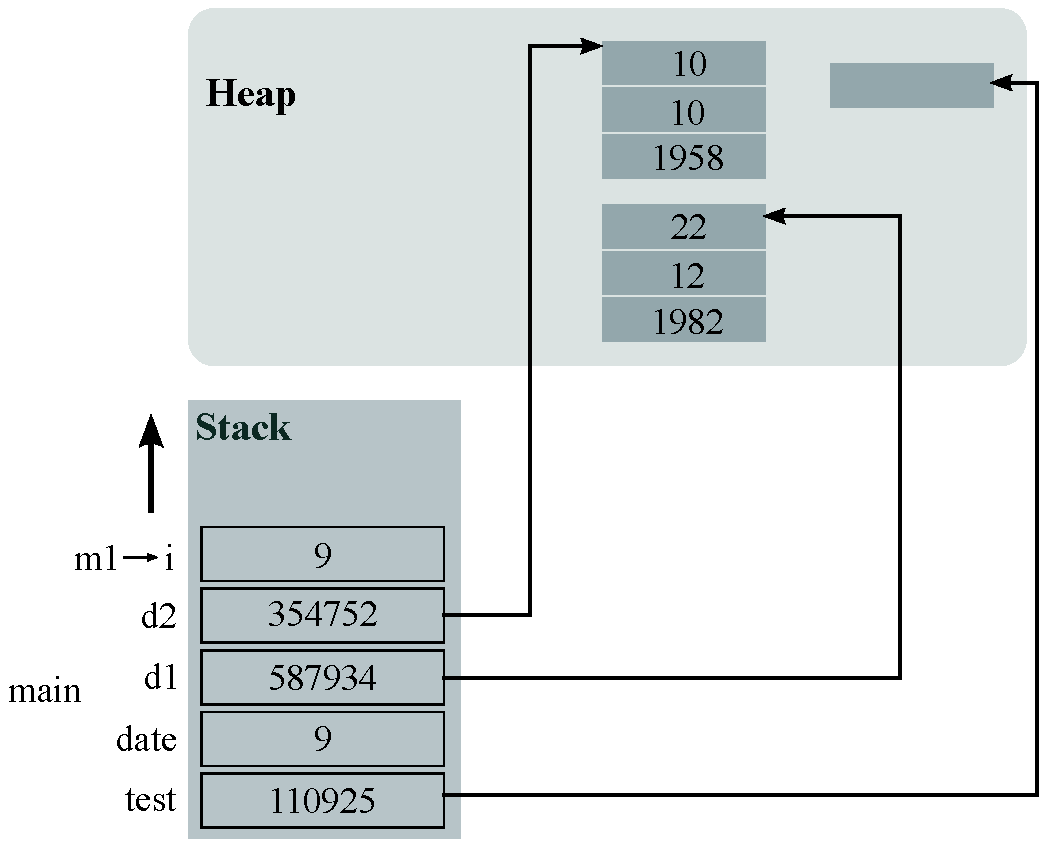
\includegraphics[width=\textwidth]{images/Java-memory-allocation/fig02.pdf}
  \end{minipage}
\end{figure}

\begin{figure}[htb]
  \begin{minipage}[t]{0.5\linewidth}
    \centering
    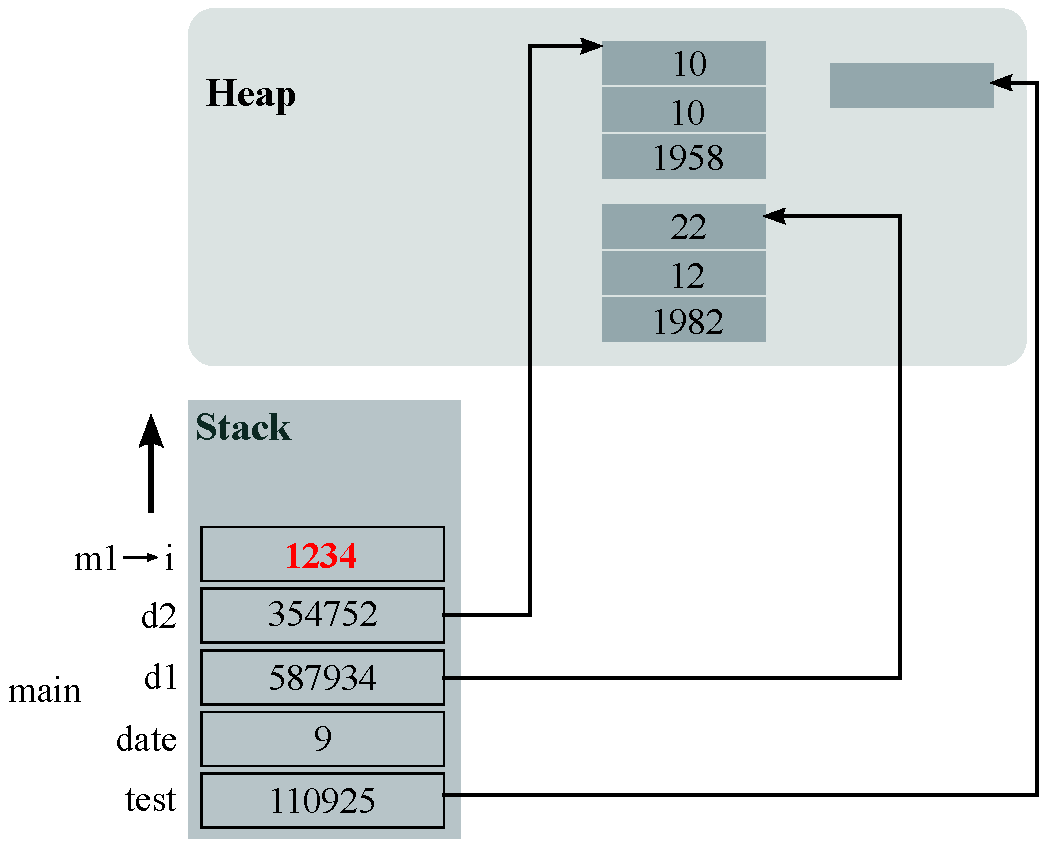
\includegraphics[width=\textwidth]{images/Java-memory-allocation/fig03.pdf}
  \end{minipage}%
  \begin{minipage}[t]{0.5\linewidth}
    \centering
    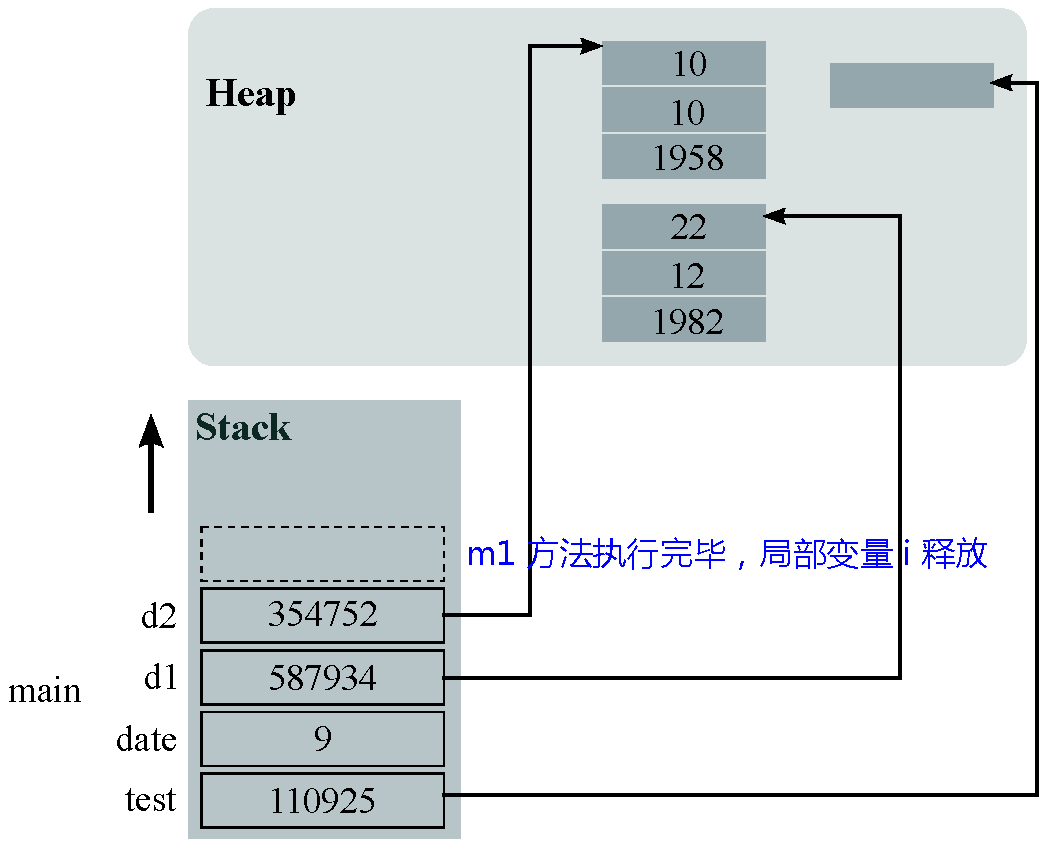
\includegraphics[width=\textwidth]{images/Java-memory-allocation/fig04.pdf}
  \end{minipage}
\end{figure}

\begin{figure}[htb]
  \begin{minipage}[t]{0.5\linewidth}
    \centering
    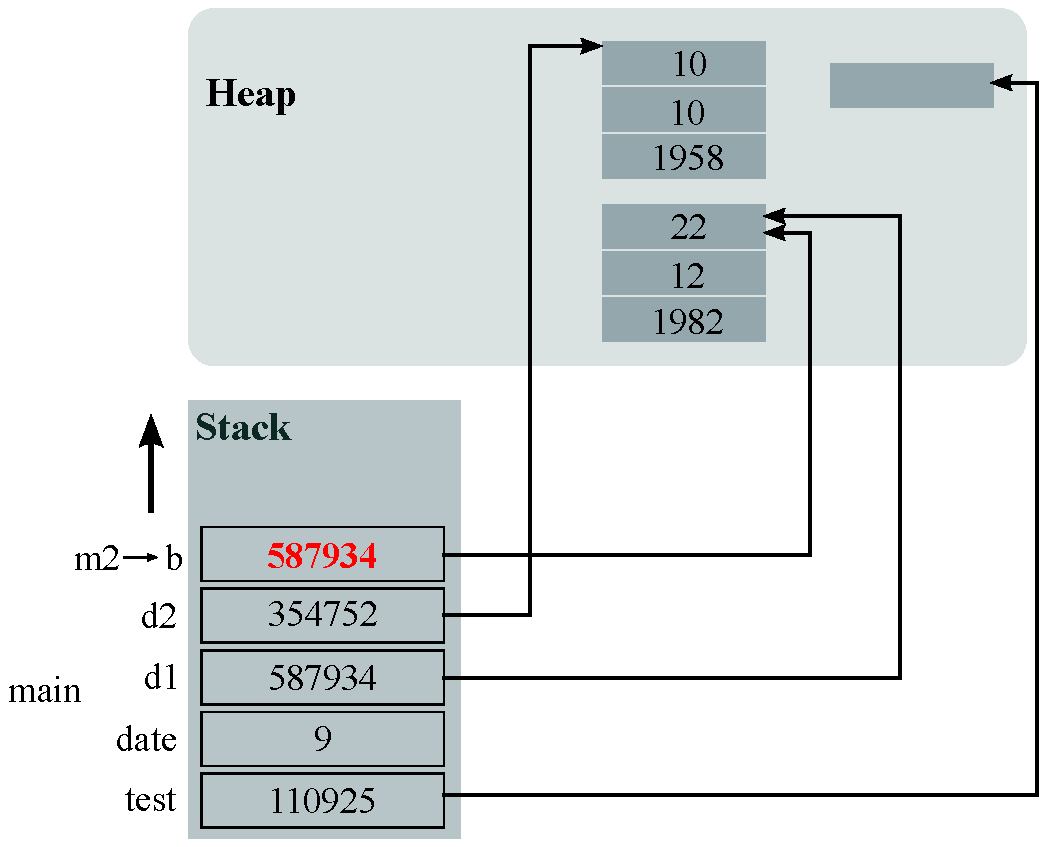
\includegraphics[width=\textwidth]{images/Java-memory-allocation/fig05.pdf}
  \end{minipage}%
  \begin{minipage}[t]{0.5\linewidth}
    \centering
    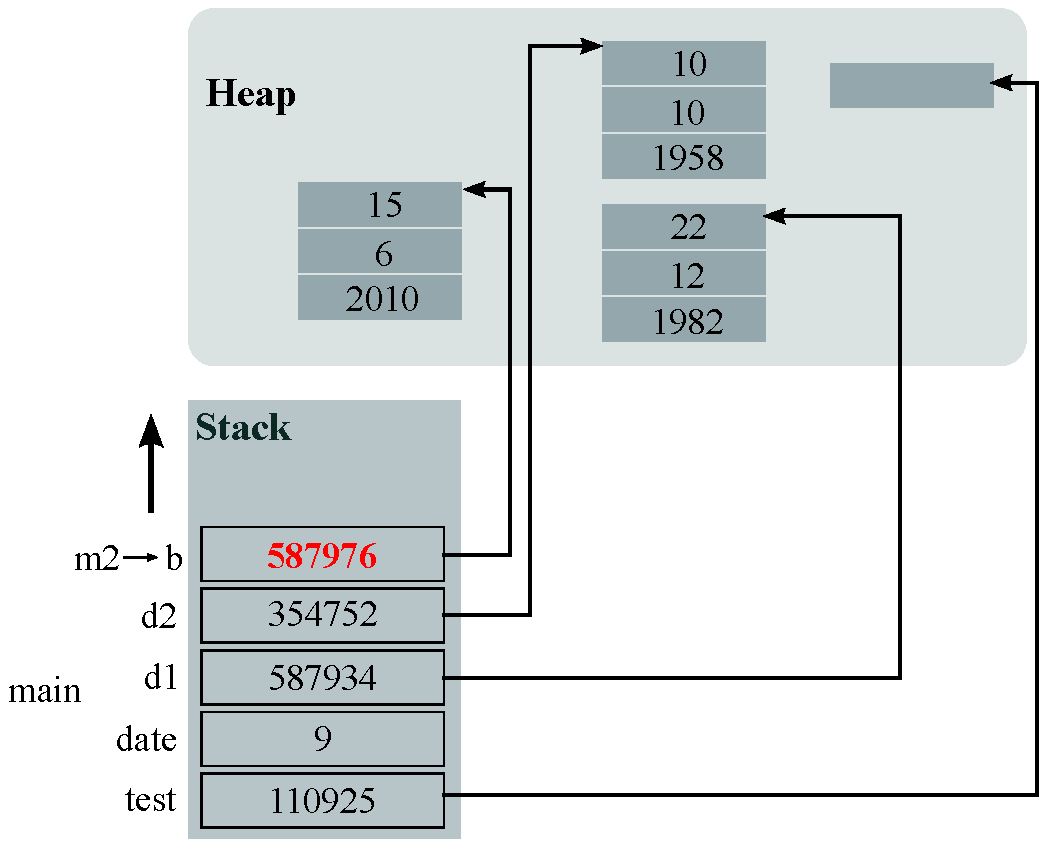
\includegraphics[width=\textwidth]{images/Java-memory-allocation/fig06.pdf}
  \end{minipage}
\end{figure}

\subsection{Java程序运行内存分析小结}

\begin{itemize}
\item 基本类型和引用类型,二者作为局部变量时都存放在栈中。
\item 基本类型直接在栈中保存值,引用类型在栈中保存一个指向堆区的指针,
  真正的对象存放在堆中。
\item 作为参数时基本类型就直接传值,引用类型传指针。
\end{itemize}

\notice{注意什么是对象}

\begin{javaCode}
  MyClass a = new MyClass();
\end{javaCode}

此时a是指向对象的指针,而不能说a是对象。指针存储在栈中,对象存储在堆中,
操作实例实际上是通过指针间接操作对象。多个指针可以指向同一个对象。

\begin{itemize}
\item {\hei\Red 栈中的数据和堆中的数据销毁并不是同步的。}方法一旦执行结
    束,栈中的局部变量立即销毁,但是堆中对象不一定销毁。因为可能有其
    他变量也指向了这个对象,直到栈中没有变量指向堆中的对象时,它才销
    毁;而且还不是马上销毁,要等垃圾回收扫描时才可以被销毁。
\item {\hei\Red 栈、堆、代码段、数据段等都是相对于应用程序而言的。}每一
    个应用程序都对应唯一的一个JVM实例,每一个JVM实例都有自己的内存区
    域,互不影响,并且这些内存区域是该JVM实例所有线程共享的。
\end{itemize}

\section{Java内存管理建议}

\subsection{Java垃圾回收机制} 

{\hei\Blue JVM的垃圾回收机制(GC)决定对象是否是垃圾对象,并进行回收。}垃圾回收机制的特点包括:

\begin{itemize}
\item 垃圾内存并不是用完了马上就被释放,所以会产生内存释放不及时的现象,
  从而降低内存的使用效率。而当程序庞大的时候,这种现象更为明显。
\item 垃圾回收工作本身需要消耗资源,同样会产生内存浪费。
\end{itemize}

JVM中的对象生命周期一般分为7个阶段:\ding{182}创建阶段、\ding{183}应用
阶段、\ding{184}不可视阶段、\ding{185}不可到达阶段、\ding{186}可收集阶
段、\ding{187}终结阶段、\ding{188}释放阶段。

Java需要内存管理,在JVM中运行的对象的整个生命周期中,进行人为的内存管理是必要的,主要原因体现在:

\begin{itemize}
\item 虽然JVM已经代替开发者完成了对内存的管理,但是硬件本身的资源是有限的。
\item 如果Java的开发人员不注意内存的使用依然会造成较高的内存消耗,导致性能的降低。
\end{itemize}

\subsection{JVM内存溢出和参数调优}

\notice{当遇到OutOfMemoryError时该如何做?}

\begin{itemize}
\item 常见的OOM(Out Of Memory)内存溢出异常,就是堆内存空间不足以存放
  新对象实例时导致。
\item 永久区内存溢出相对少见,一般是由于需要加载海量的Class数据,超过了
  非堆内存的容量导致。通常出现在Web应用刚刚启动时。因此Web应用推荐使用
  预加载机制,方便在部署时就发现并解决该问题。
 \item 栈内存也会溢出,但是更加少见。
\end{itemize}

对内存溢出的处理方法不外乎这两种:\ding{182} 调整JVM内存配置;\ding{183} 优化代码。

创建阶段的JVM内存配置优化需要关注以下项:

\begin{description}
\item[堆内存优化] 调整JVM启动参数 -Xms -Xmx -XX:newSize -XX:MaxNewSize,
  如调整初始堆内存和最大对内存 -Xms256M -Xmx512M。 或者调整初始New
  Generation的初始内存和最大内存 -XX:newSize=128M -XX:MaxNewSize=128M。
\item[永久区内存优化] 调整PermSize参数,如 -XX:PermSize=256M
  -XX:MaxPermSize=512M。
 \item[栈内存优化] 调整每个线程的栈内存容量,如 -Xss2048K。
\end{description}

\subsection{内存优化的小示例}

\subsubsection{减少无谓的对象引用创建}

\samp{Test 1}

\begin{javaCode}
  for(int i=0; i<10000; i++) {
    Object obj = new Object(); 
  }
\end{javaCode}

\samp{Test 2}

\begin{javaCode}
  Object obj = null; 
  for( int i=0; i<10000; i++) {
    obj = new Object(); 
  }
\end{javaCode}

\descript{内存性能分析}
  
{\small\kai Test 2比Test 1的性能要好。两段程序每次执行for循环都要创建一
  个Object的临时对象,JVM的垃圾回收不会马上销毁但这些临时对象。相对
  于Test 1,Test 2则只在栈内存中保存一份对象的引用,而不必创建大量新临
  时变量,从而降低了内存的使用。}


\subsubsection{不要对同一对象初始化多次}

\begin{javaCode}
  public class A { 
    private Hashtable table = new Hashtable(); 
    public A() { 
      table = new Hashtable();
    }
  }
\end{javaCode}

\descript{内存性能分析}

{\small\kai 上述代码new了两个Hashtable,但是却只使用了一个,另外一个则
  没有被引用而被忽略掉,浪费了内存。并且由于进行了两次new操作,也影响了
  代码的执行速度。另外,不要提前创建对象,尽量在需要的时候创建对象。}

\subsection{对象其他生命周期阶段内存管理}

\begin{description}
\item[应用] 即该对象至少有一个引用在维护它。
\item[不可视] 即超出该变量的作用域。\\{\kai 因为JVM GC并不是马上进行回
    收,而是要判断对象是否被其他引用维护。所以,如果我们在使用完一个对
    象以后对其进行obj = null或者obj.doSomething()操作,将其标记为空,则
    帮助JVM及时发现这个垃圾对象。}
\item[不可到达] 即在JVM中找不到对该对象的直接或者间接的引用。
\item[可收集,终结,释放] 垃圾回收器发现该对象不可到达,finalize方法已
  经被执行,或者对象空间已被重用的时候。
\end{description}

\subsubsection{Java的finalize()方法}

Java所有类都继承自Object类,而finalize()是Object类的一个函数,该函数
在Java中类似于C++的析构函数(仅仅是类似)。一般来说可以通过重
载finalize()的形式来释放类中对象。

\begin{javaCode}
  public class A { 
    public Object a; 

    public A() { 
      a = new Object() ;
    } 
    
    protected void finalize() throws java.lang.Throwable { 
      a = null; // 标记为空,释放对象 
      super.finalize(); // 递归调用超类中的 finalize 方法
    }
  } 
\end{javaCode}

什么时候finalize()被调用由JVM来决定。{\hei\Blue 尽量少用finalize()函
  数,finalize()函数是Java提供给程序员一个释放对象或资源的机会。但它会
  加大GC的工作量,因此尽量少采用finalize方式回收资源。}

\begin{itemize}
\item 一般的,纯Java编写的Class不需要重写finalize()方法,因为Object已
  经实现了一个默认的,除非我们要实现特殊的功能。
\item 用Java以外的代码编写的Class(比如JNI、C++的new方法分配的内存),
  垃圾回收器并不能对这些部分进行正确的回收,这就需要我们覆盖默认的方
  法来实现对这部分内存的正确释放和回收。
\end{itemize}

\newpage
\section*{实验设计}
\sline